\documentclass[12pt,a4paper]{article}
\usepackage[utf8]{inputenc}
\usepackage[german]{babel}
\usepackage[T1]{fontenc}
\usepackage{times}
\usepackage{url}
\usepackage{setspace}
\usepackage{pbox}
\usepackage{graphicx}
\usepackage{adjustbox}
\usepackage{enumerate}
\usepackage{amsmath}
\usepackage{subcaption}
\usepackage{amsfonts}
\usepackage{amssymb}
\usepackage{float}
\usepackage{stix}
\usepackage[dvipsnames]{xcolor}
\newcommand{\red}[1]{\textcolor{red} {#1}}
\newcommand{\blue}[1]{\textcolor{blue} {#1}}
\newcommand{\green}[1]{\textcolor{ForestGreen} {#1}}
\newcommand{\yellow}[1]{\textcolor{yellow} {#1}}
\newcommand{\magenta}[1]{\textcolor{magenta} {#1}}
\newcommand{\cyan}[1]{\textcolor{cyan} {#1}}
\newcommand{\orange}[1]{\textcolor{orange} {#1}}
\newcommand{\nl}{\\[0.1cm]}
\newcommand{\floor}[1]{\lfloor #1 \rfloor}
\title{Zusammenfassung Software-orientierte Informatik}
\author{Henrik Tscherny}
\begin{document}
\maketitle
\tableofcontents

\section{Systeme}
Ein System ist ein natürliches oder künstliches Gebilde, welches aus Eingangssignalen ($E$) ein Ausgangssignal ($A$) macht. Das System besitzt zudem einen inneren Zustand, der durch Zustandsgrößen ($\vec{Z}$) beschrieben wird. Eine Systemfunktion ($F$) legt fest wie das Eingangssignal in das Ausgangssignal umgewandelt wird ($\vec{A} = F(\vec{E}, \vec{Z},...)$)

\paragraph{Statische Systeme}
Der Output zum Zeitpunkt t ($y(t)$) ist nur von dem zu gleichen Zeitpunkt am Input anliegenden Wert ($x(t)$) abhängig. Innere Zustände ($\vec{Z}$) sind egal. die dazugehörige Funktion $y=f(x)$ nennt man statische Kennlinie.

\paragraph{Dynamische Systeme}
Der Output ($y(t)$) ist von dem am Input anliegenden Signal ($x(t)$) und dem inneren Zustand des Systems ($\vec{Z}$) abhängig. Dabei kann man sich den inneren Zustand als eine Art Gedächtnis vorstellen

\paragraph{Lineare Systeme}
Ein System ist linear, wenn der Überlagerungssatz/Superpositionsprinzip gilt, bzw nicht-linear falls dieser nicht gilt, d.h. Stellt man den Input als die Summe von zwei verschiedenen Inputs dar, so kann man auch den Output als die Summe der beiden Outputs darstellen.\\
$f(x_1 + x_2) = f(x_1) + f(x_2) \Rightarrow y(t) = f(x_1(t) + x_2(t)) = f(x_1(t)) + f(x_2(t))$\\
lineare Systeme werden durch lineare Differenzialgleichungen mit konstanten Koeffizienten beschrieben
\begin{figure}[H]
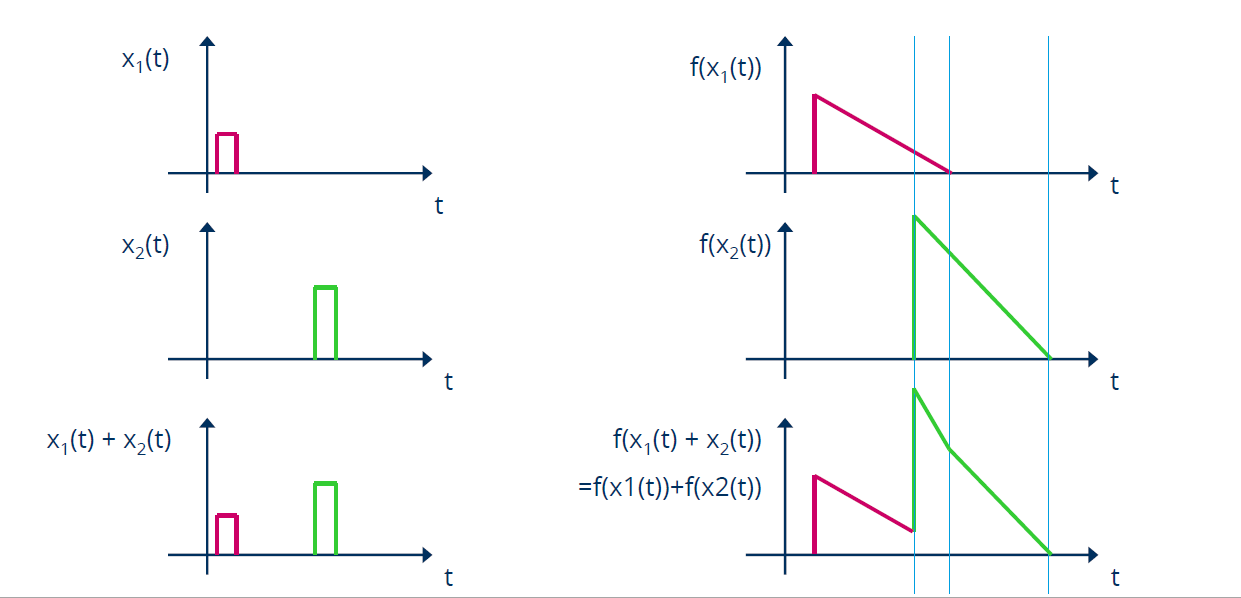
\includegraphics[scale=0.3]{./resources/linear-system.png}
\caption{Veranschaulichung des Superpositionsprinzips}
\end{figure}

\paragraph{Zeit(in)variante Systeme}
Ändern sich die Systemeigenschaften sich nicht mit der Zeit, d.h. es gilt das Verschiebungsprinzip ($y(t-t_0) = f(x(t-t_0))$), ist das System zeitinvariant, andernfalls ist es zeitvariant

\paragraph{Kausales System}
Der Output ist nur von den aktuellen und vergangenen Inputs abhängig, Sprung- und Impulsantwort sind gleich 0 für $t < 0$, gilt dies nicht ist das System akausal.
\begin{itemize}
\item schwach kausal
\begin{itemize}
\item reagiert auf Input x immer mit gleichem Output y
\end{itemize}
\item stark kausal
\begin{itemize}
\item reagiert auf ähnlichen Input x mit ähnlichem Output y
\end{itemize}
\end{itemize}

\subsection{Verknüpfung von Systemen}

\paragraph{Reihenschaltung}
\hspace{1pt}
\begin{figure}[H]
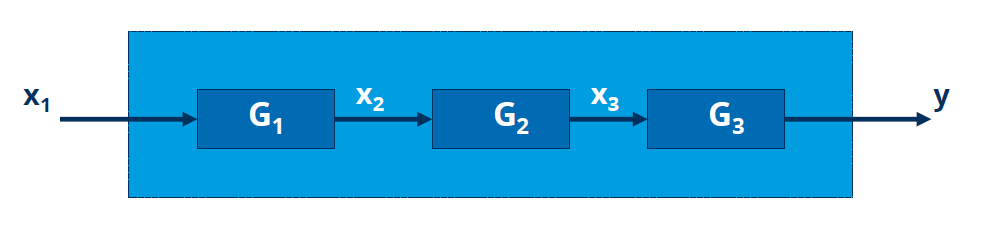
\includegraphics[scale=0.5]{./resources/reihenschaltung.png}
\end{figure}
\begin{tabular}{|c|c|}
\hline
\textbf{statisches System} & \textbf{dynamisches System} \\
$\displaystyle k_{ges} = \prod_{i=1}^n k_i = \frac{\text{output}}{\text{input}}$ & $\displaystyle G_{ges}(f) = \prod_{i=1}^n G_i(f) = \frac{\text{input}(f)}{\text{output}(f)}$ \\
\hline
$G_i = k_i$: statische Übertragungsfaktor & $G_i(f)$: Übertragungsfunktion des Teilsystems i \\
\hline
\end{tabular}
\newpage
\paragraph{Parallelschaltung}
\hspace{1pt}
\begin{figure}[H]
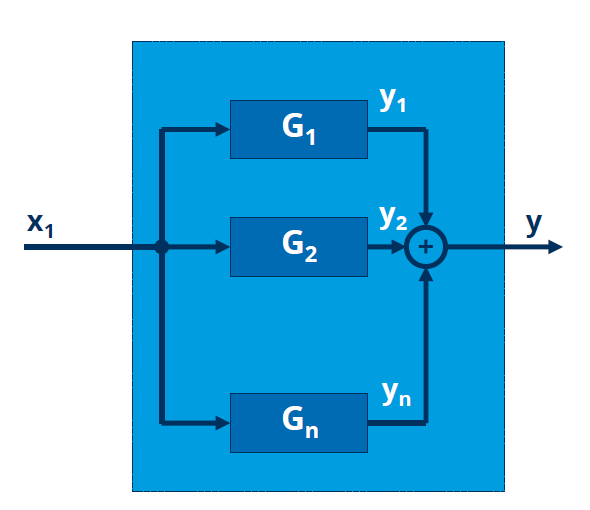
\includegraphics[scale=0.5]{./resources/parallelschaltung.png}
\end{figure}
\begin{tabular}{|c|c|}
\hline
\textbf{statisches System} & \textbf{dynamisches System} \\
$\displaystyle k_{ges} = \sum_{i=1}^n k_i$ & $\displaystyle G_{ges}(f) = \sum_{i=1}^n G_i(f)$\\
\hline
$G_i = k_i$: statische Übertragungsfaktor & $G_i(f)$: Übertragungsfunktion des Teilsystems i \\
\hline
\end{tabular}

\paragraph{Rückkopplungsschaltung}
\hspace{1pt}
\begin{figure}[H]
\includegraphics[scale=0.5]{./resources/rückkopplungsschaltung.png}
\end{figure}
\begin{tabular}{|c|c|}
\hline
\textbf{statisches System} & \textbf{dynamisches System} \\
$\displaystyle k_{ges} = \frac{y}{x} = \frac{k_1}{1 \pm k_1 k_2}$ & $\displaystyle G_{ges}(f) = \frac{G_1(f)}{1 \pm G_1(f)G_2(f)}$\\
\hline
\end{tabular}

\subsection{Grundsysteme}
\begin{tabular}{|c|c|c|}
\hline
Type & Differenzialgleichung & Differenzengleichung\\
\hline
\begin{tabular}{c}
Proportionalsystem (P)\\
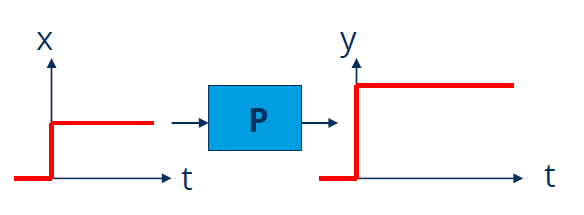
\includegraphics[scale=0.3]{./resources/p-sys.png} 
\end{tabular} & $\frac{dy}{dx} = K_p$ & $y(i) = K_p x(i)$\\
\hline
\begin{tabular}{c}
Integralsystem (I)\\
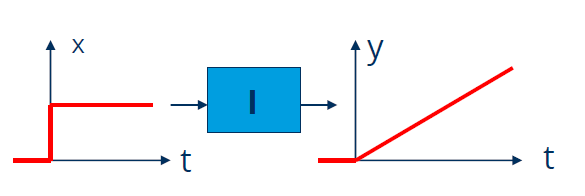
\includegraphics[scale=0.3]{./resources/i-sys.png}
\end{tabular} & \begin{tabular}{c}
$\frac{dy}{dt} = K_I x(t)$\\
$\displaystyle y(t) = K_I \int_0^t x(\tau) d\tau$
\end{tabular} & $y(i) = TK_I x(i) + y(i-1)$ \\
\hline
\begin{tabular}{c}
Differentialsystem (D) \\
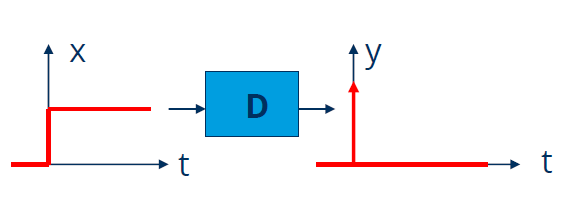
\includegraphics[scale=0.3]{./resources/d-sys.png}
\end{tabular} & $\frac{dx}{dt}K_D = y(t)$ & $y(i) = \frac{K_D}{T}(x(i)-x(i-1))$\\
\hline
\begin{tabular}{c}
Totzeitsystem ($T_t$)\\
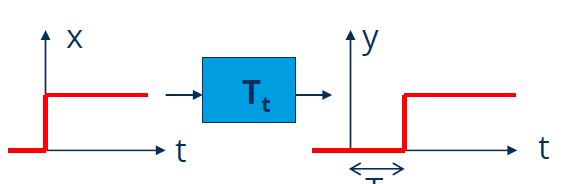
\includegraphics[scale=0.3]{./resources/tt-sys.png}
\end{tabular} & $y(t) = x(t-T_t)$ & \begin{tabular}{c}
$y(i) = x(i-n)$\\
$n=\frac{T_t}{T}$
\end{tabular}\\
\hline
\begin{tabular}{c}
Verzögerunssystem ($T_1$)\\
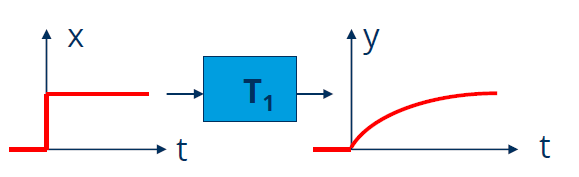
\includegraphics[scale=0.3]{./resources/t1-sys.png}
\end{tabular} & $\frac{dy}{dt}T_1 + y(t) = x(t)$ & \begin{tabular}{c}
$y(i) = (1-\alpha)x(i) +\alpha y(i-1)$\\
$\alpha=\frac{T_1}{T+T_1}$
\end{tabular}\\
\hline
\end{tabular}

\section{Faltung/Konvolution}
Die Faltung beschriebt einen mathematischen Operator ($\ast$) welcher für zwei Funktionen f und g eine dritte Funktion $f \ast g$ liefert.\nl
$\displaystyle (f\ast g)(x) = \int_{\mathbb{R^n}} f(\tau) g(x-\tau)d\tau$\nl
Intuitiv kann man sich die Faltung von zwei Funktionen f und g so vorstellen, dass man die Funktion g entlang der x-Achse schiebt (daher $x-\tau$) und dabei diese über die Funktion f hinweg schiebt. Dabei berechnet man dann in jedem Schritt die Fläche in welcher sich die beiden Funktionen überlappen. Der Flächeninhalt der Überlappung ist dann der Funktionswert der Funktionswert der Funktion $(f \ast g) (x)$. Die Funktion f wird also mit der Funktion g an jedem Punkt x gewichtet.
\flushleft

\textbf{Eigenschaften der Faltung}:
\begin{itemize}
\item Kommutativität: $f \ast g = g \ast f$
\item Assoziativität: $f \ast (g \ast h) = (f \ast g) \ast h$
\item Distributivität: $f \ast (g+h) = (f \ast g) + (f \ast h)$
\item Assoziativ mit Skalarmultiplikation: $a(f\ast g) = (af)\ast g = f \ast (ag)$
\end{itemize}
\flushleft
Für den zeitdiskreten Fall gibt es äquivalent zum Faltungsintegral die Faltungssumme:\nl
$\displaystyle f(kT) \ast g(kT) = \begin{cases} 0 & k<0 \\
\displaystyle \sum_{j=0}^k f((k-j)T)g(jT) & k \geq 0
\end{cases}$\nl
$k \in \mathbb{Z}$ , T: Abtastperiode

\paragraph{Stabilität}
Ein System ist \textbf{BIBO-stabil}, wenn es für jeden beschränkten Input Wert auch nur maximal einen beschränkten 
Output wert liefert\nl
\begin{itemize}
\item zeitkontinuierlich: $\displaystyle \int_{-\infty}^{+\infty} |g(t)|dt < \infty$
\item zeitdiskret: $\displaystyle \sum_{-\infty}^{+\infty} |g(kT)|T < \infty$
\end{itemize}

\subsection{Beispiel}
Faltung der Rechteckfunktion mit sich selbst:\nl

\begin{minipage}{\linewidth}
\centering
\begin{minipage}{0.45\linewidth}
\begin{figure}[H]
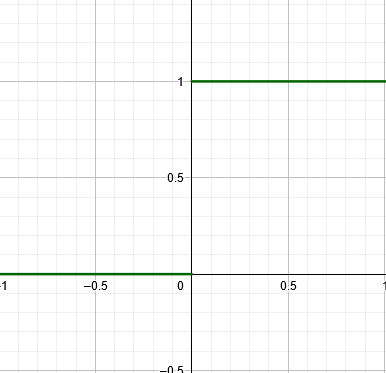
\includegraphics[width=0.9\linewidth]{./resources/einheitssprung_funktion.png}
\end{figure}
\end{minipage}
\hspace{0.05\linewidth}
\begin{minipage}{0.45\linewidth}
\begin{figure}[H]
Sei $u(x) = \displaystyle \begin{cases} 0, & x<\tau \\ 1, & x\geq \tau \end{cases}$\\
der Einheitssprung beginnend ab\\ $x = \tau$
\end{figure}
\end{minipage}
\end{minipage}
\nl

\begin{minipage}{\linewidth}
\centering
\begin{minipage}{0.45\linewidth}
\begin{figure}[H]
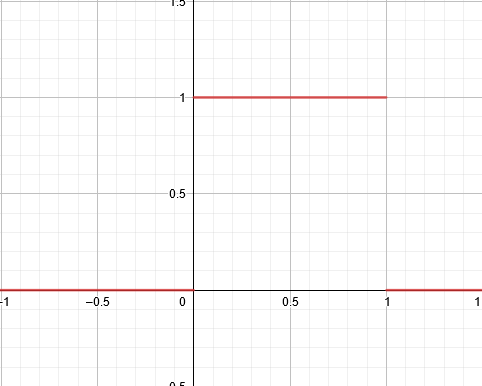
\includegraphics[width=0.9\linewidth]{./resources/rechteck_funktion.png}
\end{figure}
\end{minipage}
\hspace{0.05\linewidth}
\begin{minipage}{0.45\linewidth}
\begin{figure}[H]
Stelle die Rechteckfunktion als die Differenz von zwei Einheitssprüngen dar\\
$r(x) = u(x) - u(x-1)$
\end{figure}
\end{minipage}
\end{minipage}
\nl


\begin{minipage}{\linewidth}
\centering
\begin{minipage}{0.45\linewidth}
\begin{figure}[H]
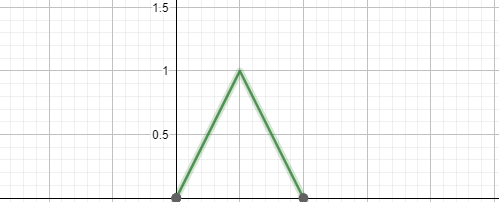
\includegraphics[width=\linewidth]{./resources/rechteck_faltung.png}
\end{figure}
\end{minipage}
\hspace{0.05\linewidth}
\begin{minipage}{0.45\linewidth}
\begin{figure}[H]
Faltung mit sich selbst: $(r\ast r)(x) = \displaystyle \int_{\mathbb{R}^n} r(\tau)r(x-\tau)d\tau = \begin{cases} 0,& x<0 \\ 2x, & 0 \leq x \leq 0.5 \\ -2(x-1), & 0.5 \leq x \leq 1 \end{cases}$
\end{figure}
\end{minipage}
\end{minipage}
\nl
Man kann leicht sehen, dass der Wert von $(f \ast f) (0.5) = 1$, da sich dort die beiden Rechteckfunktionen exakt überlagern, somit ist die Fläche gleich 1


\section{Fourier}
In diesem Kapitel fassen wir Techniken zusammen, welche es erlauben eine gegebene Funktion f in ein Spektrum, bzw. in eine Spektralfunktion zu zerlegen. Man kann die Zerlegung am Beispiel eines gespielten Akkords veranschaulichen. Jeder Ton des Akkords ist eine Schwingung mit seiner eigenen Frequenz. Diese Frequenzen überlagern sich dann alle zusammen zu einer neuen Schwingung und bilden so den Akkord. Man kann nun FT benutzten um aus der Akkordschwingung die Schwingungen der einzelnen Noten zurückzugewinnen. Die Spektralfunktion welche man erhält, hat dann für jeden Ton des Akkords einen Ausschlag mit x=Frequenz. und mit der Höhe je nachdem wie laut, d.h. wie groß die Amplitude des jeweiligen Tons ist y=Amplitude.\nl
\subsection{Fourier Reihe}
Die Fourier Reihe ist eine Funktion welche aus einer unendlichen Summe von gewichteten Sinus- und Kosinusschwingungen besteht. $\displaystyle f(t) = \frac{a_0}{2} + \sum_{n=1}^\infty (a_n \cdot \cos (n\omega t) + b_n\cdot \sin(n\omega t))$\nl
Man kann so eine periodische Funktion f mit Periode $T>0$, als eine Reihe von Sinus- und Kosinusfunktionen darstellen. Die Frequenzen der einzelnen Funktionen müssen dabei ganzzahlige Vielfache der Grundfrequenz $\omega = \frac{2\pi}{T}$ sein, da sonnst die Grundperiodizität verletzt wird.
\begin{figure}[H]
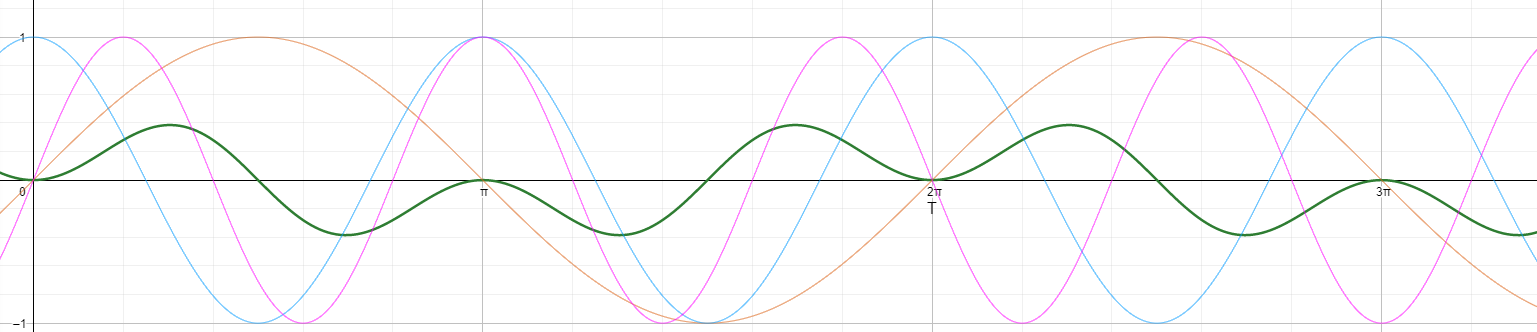
\includegraphics[width=\textwidth]{./resources/grundperiode.png}
\caption{$\cyan{\cos(2x)}$, $\orange{\sin(x)}$, $\magenta{\sin(2.5x)}$}
\end{figure}
Die \green{grüne} Funktion kann unmöglich aus der \magenta{pinken} Funktion bestehen, da diese die Grundperiodizität derer verletzt.\\
$\frac{4\pi}{3} = T_{\magenta{pink}} \nmid 2\pi = T_{\green{gr"un}}$\nl
Jedoch \textbf{kann} die \green{grüne} Funktion aus der \orange{orangenen} oder der \cyan{blauen} Funktion bestehen.\\$\pi = T_{\cyan{blau}} \mid 2\pi = T_{\orange{orange}} \mid 2\pi = T_{\green{gr"un}}$\nl
Außerdem ist die Entwicklung nur möglich wenn die Dirichletschen Bedigungen erfüllt sind:
\begin{itemize}
\item Das Periodenintervall lässt sich in endlich viele stetig-monotone Teilintervalle zerlegen
\item An Diskontinuitäten existiert der rechts und links-seitige Grenzwert, d.h. es kommen nur endliche Sprünge in Betracht (z.B. nicht der Fall für $\tan(x)$
\end{itemize}
Die Koeffizienten der Entwicklung von f können dann wie folgt berechnet werden:\nl
\begin{itemize}
\item $\displaystyle a_0 = \frac{1}{T} \int_c^{c+T} f(t)\, dt$ (Absolut-Anteil)
\item $\displaystyle a_n = \frac{2}{T} \int_c^{c+T} f(t)\cdot \cos(n\omega t)\,dt$ (Cosinus-Anteil)
\item $\displaystyle b_n = \frac{2}{T} \int_c^{c+T} f(t)\cdot \sin(n\omega t)\,dt$ (Sinus-Anteile)
\item c ist die Verschiebung des Intervalls und kann beliebig gewählt werden (auch $c=0$)
\end{itemize}
Note: Ist die Funktion nicht über eine ganze Periode integrierbar, z.B. wegen einer Sprungstelle, dann müssen mehrere Integrale benutzt werden, jeweils für die Teile in denen die Funktion integriert Werden kann\\
Trägt man die $a_n$'s bzw. $b_n$'s in Abhängigkeit der Frequenz ab so erhält man eine dazugehörige \textbf{diskrete Spektralfunktion}\\
\begin{figure}[H]
\begin{subfigure}{0.4\textwidth}
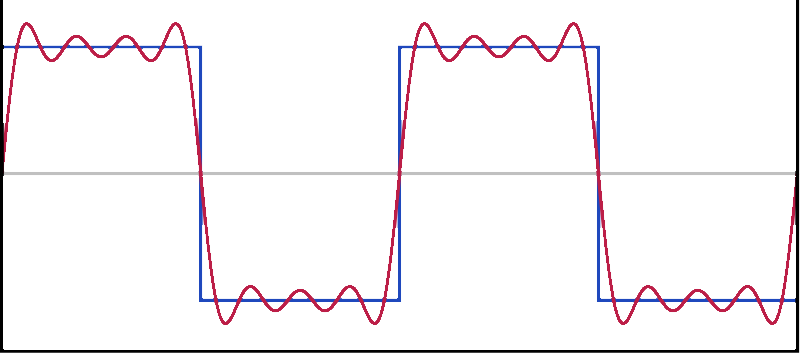
\includegraphics[width=\textwidth]{./resources/rec_sins.png}
\caption{4x approximierte Rechteckfunktion}
\end{subfigure}
\hfill
\begin{subfigure}{0.4\textwidth}
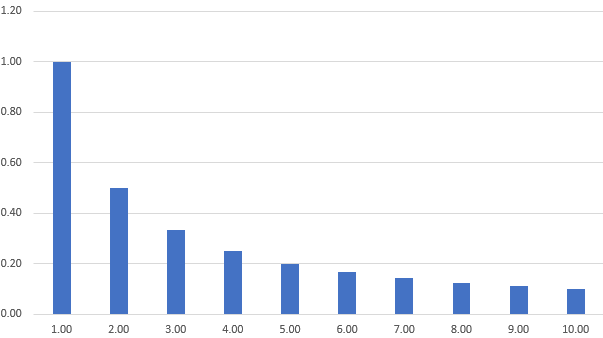
\includegraphics[width=\textwidth]{./resources/freq_diag_rec.png}
\caption{Spektrum der $a_n$'s bis $n=10$}
\end{subfigure}
\end{figure}
\textbf{Herleitung der Koeffizientenformeln}:\nl
Um die Gleich für Koeffizienten zu erhalten benutzen wir die Orthogonalitätsrelationen der trigonometrischen Funktionen, welche wie folgt lauten:
\begin{enumerate}
\item $\displaystyle \int_0^{2\pi} \cos mx \cdot \cos nx \,dx = \begin{cases}\pi ,& m=n\\0 ,& m\neq n\end{cases}$
\item $\displaystyle \int_0^{2\pi} \sin mx \cdot \sin nx \,dx = \begin{cases}\pi ,& m=n\\0 ,& m\neq n\end{cases}$
\item $\displaystyle \int_0^{2\pi} \cos mx \cdot \sin nx \,dx = \int_0^{2\pi} \sin mx \cdot \cos nx \,dx = 0$
\end{enumerate}
Nun machen wir folgende Umformung:\nl
$\displaystyle \green{\int_0^{2\pi}} f(t)\, \green{\sin mt \, dt}$
$\displaystyle = \green{\int_0^{2\pi}} \bigg( \frac{a_0}{2} + \sum_{n=1}^\infty (a_n \cdot \cos n\omega t + b_n\cdot \sin n\omega t)\bigg)\, \green{\sin mt\, dt}$
\begin{itemize}
\item $\displaystyle \int_0^{2\pi} \frac{a_0}{2} \cdot \sin mt \, dt = 0$, \quad Sinus über eine Periode mal Konstante = 0
\item $\displaystyle \int_0^{2\pi} a_n \cdot \cos nt \cdot  \sin mt \, dt = 0$, \quad$\rightarrow$ Folgt aus Gleichung (3)
\item $\displaystyle \int_0^{2\pi} b_n \cdot \sin nt \cdot  \sin mt \, dt = b_m \pi$, \quad$\rightarrow$ Folgt aus Gleichung (2)\\
\end{itemize}
daraus folgt:
$\displaystyle b_n = \frac{1}{\pi} \int_0^{2\pi} f(t) \sin nt \, dt$\nl
$\displaystyle \green{\int_0^{2\pi}} f(t)\, \green{\cos mt \, dt}$
$\displaystyle = \green{\int_0^{2\pi}} \bigg( \frac{a_0}{2} + \sum_{n=1}^\infty (a_n \cdot \cos n\omega t + b_n\cdot \sin n\omega t)\bigg)\, \green{\cos mt\, dt}$
\begin{itemize}
\item $\displaystyle \int_0^{2\pi} \frac{a_0}{2} \cdot \cos mt \, dt = 0$, \quad Cosinus über eine Periode mal Konstante = 0
\item $\displaystyle \int_0^{2\pi} b_n \cdot \sin nt \cdot  \cos mt \, dt = 0$, \quad$\rightarrow$ Folgt aus Gleichung (3)
\item $\displaystyle \int_0^{2\pi} a_n \cdot \cos nt \cdot  \cos mt \, dt = 0$, \quad$\rightarrow$ Folgt aus Gleichung (1)
\end{itemize}
daraus folgt:
$\displaystyle a_n = \frac{1}{\pi} \int_0^{2\pi} f(t) \cos mt \, dt$\nl
$\displaystyle \green{\int_0^{2\pi}} f(t)\, \green{1 \, dt}$
$\displaystyle = \green{\int_0^{2\pi}} \bigg( \frac{a_0}{2} + \sum_{n=1}^\infty (a_n \cdot \cos n\omega t + b_n\cdot \sin n\omega t)\bigg)\, \green{1\, dt}$
\begin{itemize}
\item $\displaystyle \int_0^{2\pi} 1 \cdot \cos nt = 0$ \quad Cosinus über eine Periode = 0
\item $\displaystyle \int_0^{2\pi} 1 \cdot \sin nt = 0$ \quad Sinus über eine Periode = 0
\item $\displaystyle \int_0^{2\pi} 1 \cdot \frac{a_0}{2} = \frac{a_0}{2} \cdot 2\pi = a_0 \pi$ 
\end{itemize}
daraus folgt:
$\displaystyle a_0 = \frac{1}{\pi} \int_0^{2\pi} f(t) 1\, dt$

\subsection{Fourier Transformation}
Die Fourier Transformation ist eine Erweiterung der Fourier Reihen, welche man erhält wenn man erlaubt, dass die Periode der zu approximierenden Funktion gegen unendlich geht (d.h. es muss in der Praxis keine Wiederholungen innerhalb der Funktion geben). Wie auch bei den Fourier Reihen, erhält man bei der Fourier Transformation wieder ein Spektrum welches nun jedoch \textbf{kontinuierlich} ist.

\subsubsection{Beispiel FT eines Rechteckimpulses}
Sei $f(t) = \begin{cases}1& t\in[0,1[ \\ 0&\text{else} \end{cases}$
\begin{itemize}
\item Setze $f(t)$ die Formel für FT ein\nl
$\displaystyle F(w) = \int_{-\infty}^{\infty} f(t) e^{-iwt} dt = \begin{cases} \displaystyle\int_0^1 1\cdot e^{-iwt} dt & t\in[0,1[ \\ 0 & \text{else} \end{cases}$
\item Umformung mittels partieller Integration\nl
Using: $u=1, u'=0, v'=e^{iwt}, v=\frac{-e^{-iwt}}{iw}$\nl
$\displaystyle \int_0^1 u\cdot v' = \int_0^1 1\cdot e^{-iwt} dt \Rightarrow u\cdot v - \int_0^1 u'\cdot v dt \Rightarrow 1\cdot \frac{-e^{-iwt}}{iw} - \int_0^1 0\cdot \frac{-e^{-iwt}}{iw}$\nl
$\displaystyle F(w) = \big[\frac{-e^{-iwt}}{iw}\big]^1_0 = \frac{1}{w}(e^{-iwt}-1)$
\item Berechne Real- und Imaginärteil von $F(w)$\nl
$\frac{1}{w}(e^{-iwt}-1) = \frac{1}{w}(\cos(w) - i\cdot \sin(w) -1)$\\
$=\;\frac{\cos(w)}{w} - \frac{1}{w} -\frac{i\sin(w)}{w} = \frac{\cos(w) -1 }{w} - \frac{i\sin(w)}{w}$\nl
\begin{itemize}
\item $\Re(F(w)) = \frac{\cos(w)-1}{w}$
\item $\Im(F(w)) = \frac{\sin(w)}{w}$
\end{itemize}
\end{itemize}
\begin{figure}[H]
\centering
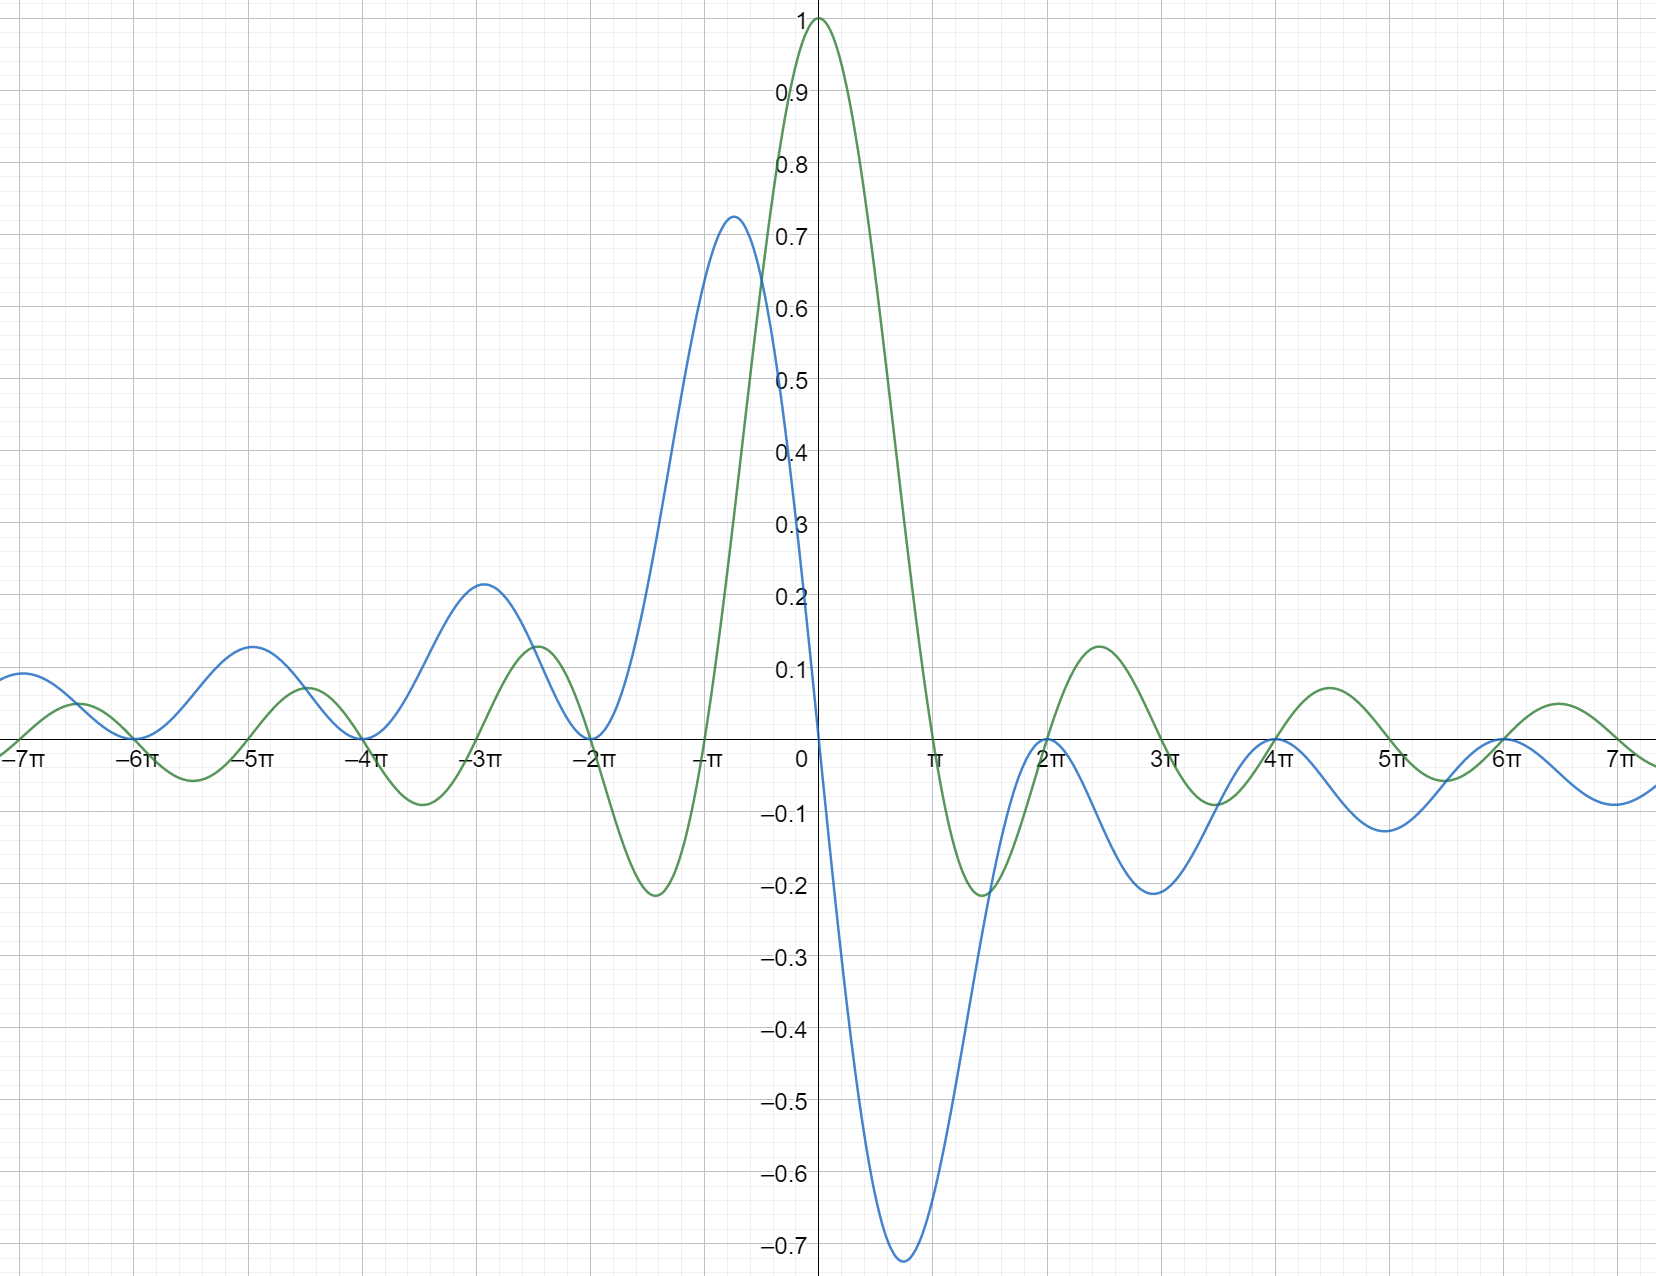
\includegraphics[scale=0.2]{./resources/ft_res.png}
\caption{$\Re(F(w))$: \blue{Blau}, $\Im(F(w))$: \green{Grün}}
\end{figure}

\end{document}